% !TEX root = BA-Bericht.tex
\chapter{Methode}\label{ch:Methode}

% Hier halten Sie fest und begründen, welches Vorgehensmodell Sie für Ihr Projekt wählen. Sie
% verweisen allenfalls auf die daraus entstandenen, konkreten Terminpläne mit Meilensteinen, welche
% z.B. unter Realisierung (Kapitel 5) oder im Anhang versorgt sind.
% Bei Projekten mit einer verlangten wissenschaftlichen Tiefe werden hier die geplanten
% Forschungsmethoden wie quantitative/qualitative Interviews, Befragungen, Beobachtungen,
% Feldexperiment etc. beschrieben und begründet.
% Warum ist in Ihrer Situation ein Interview besser als eine Umfrage? Wer soll interview werden?
% 2(Sie können bei Bedarf in Absprache mit Ihrer Betreuungsperson dazu auch ein zusätzliches
% Methodencoaching beziehen).
% Bei Engineering-Projekten halten Sie weitere einzusetzende fachliche Methoden oder Techniken fest.
% Bei einem Softwareprojekt können dies z.B. der geplante Einsatz einer Anforderungsanalyse, der
% Einsatz von Review-Techniken (Architektur-Reviews) oder bekannter Programmiertechniken sein.
% Dazu gehört auch eine Teststrategie (wo setzen Sie im Projekt Schwerpunkte betr. Testen?). Die
% eigentliche Testdurchführung ist dann unter Realisierung, im Anhang oder einem selbstständigen
% Testdokument beschrieben.

Als wissenschaftliche Methode wurde ein Experiment durchgeführt.
Als Vorgehensmodell für das Projektmanagement wurde KanBan ausgewählt.

% TODO Nach eigenen Bedürfnissen erweitern
% ------------------------------------- TEIL Wissenschaftliche Arbeiten ----------------------------------------------------


\section{Experiment}\label{sec:experiment}
% quantitaiv, ehter verhaltenswissenschaftlich als konstruktiv

% Das Experiment untersucht Kausalzusammenhängein kontrollierter Umgebung, indem
% eine Experimen-talvariable auf wiederholbare Weise manipuliert unddie Wirkung
% der Manipulation gemessen wird. DerUntersuchungsgegenstand wird entweder in
% seiner na-türlichen Umgebung (im »Feld«) oder in künstlicherUmgebung (im
% »Labor«) untersucht, wodurch wesentlichdie Möglichkeiten der Umgebungskontrolle
% beeinflusstwerden. (Balzert, S. 286)

Es soll ein Experiment durchgeführt werden, um eine quantitative Analyse durchführen zu können.
Spezifischer soll ein Laborexperiment durchgeführt werden, um die Hypothese \ref{hyp:first} zu testen.
Dabei gilt es, die drei Qualitätskriterien Messbarkeit, Wiederholbarkeit und Überprüfbarkeit zu beachten.
Damit die Performance-Experimente an I2P durchgeführt werden können, muss ein Testnetzwerk aufgebaut werden sowie eine Messanlage entwickelt werden.
% Die Konfigurationsoptionen können als unabhängige Variable gesehen werden, welche verändert werden.
% Diese haben somit auf die um die Auswirkung auf die abhängigen Variablen zu messen, wie die Latenzzeit von Nachrichten.
\parencite[S.~276]{helmut_balzert_wissenschaftliches_2017}

% \section{Prototyping}
%
% Dies ist ein Teststand der ein isoliertes I2P-Netzwerk erstellt, welches mit Messpunkten für Performance-Messungen versehen werden kann.
%
% Um jedoch ein Experiment durchführen zu können benötigt es
% eine Software. für die Ausarbeitung des Konzepts für den Teststand müssen einige Sachen erst in Software ausprobiert werden,
% um schnell zu merken, ob man auf dem richtigen Weg ist bevor zu viel Zeit vergangen ist.
% Deshalb wird zur Entwicklung des Teststands ein Prototyping Verfahren eingesetzt.
% Dabei wird ein Lösungsansatz ausprobiert. 

% \parencite{helmut_balzert_wissenschaftliches_2017}


% ------------------------------------- TEIL Ingenieurlastige Arbeiten ----------------------------------------------------
\section{Projektmanagement}\label{sec:projektinformationen}

In diesem Abschnitt wird aufgezeigt welches, Vorgehensmodell verwendet wurde und wie das Projekt abgewickelt wurde.
Auch wird aufgezeigt, wie das Projekt organisiert ist, wie die Anforderungen ermittelt wurden und welche Anforderungen es gibt.

\subsection{Vorgehensmodell}

In den Besprechungen hat sich ergeben, dass inkrementell und iterativ gearbeitet wird, so wie auch von der Aufgabenstellung vorgeschlagen (siehe Anhang~\ref{ch:assignment}).
Das Projektmanagement soll schlank gehalten werden und nicht viel Aufwand erzeugen, da alleine an dem Bericht gearbeitet wird.
Deshalb wurde Kanban als Vorgehensmodell ausgewählt.
Einige wichtige Kernpraktiken von Kanban sind hier kurz erklärt:

\begin{enumerate}
    \item \textbf{Arbeit sichtbar machen}: Arbeit muss sichtbar gemacht werden, um zu sehen wo der Arbeitsfluss im Gesamtsystem stockt.
        Auch arbeitet man bei Kanban nicht nach dem Push-Prinzip sondern dem Pull-Prinzip.
        Das heisst es wird keine Arbeit zugewiesen, sondern neue Arbeit wird abgeholt, sobald die letzte Aufgabe (oder Issue/Task) fertiggestellt wurde.
    \item \textbf{Limitiere den Work in Progress (WIP)}: Es ist schwierig ständig zwischen verschiedenen Aufgaben zu wechseln. Deshalb soll nur an einer Aufgabe auf einmal gearbeitet werden.
    Tritt bei einer Aufgabe ein Problem auf, legt man sie auf die Seite, um sie später mit jemandem anzuschauen, oder erledigt erst eine andere Aufgabe, welche eine Voraussetzung dafür ist.
    \item \textbf{Manage Flow}: Arbeitsfluss ist wichtig in Kanban.
    Die Aufmerksamkeit soll auf Engpässe oder Blockaden im System gelegt werden.
    Dabei hilft es, zu unterscheiden, was für verschiedene Arbeitstypen das Team erledigen muss, und diesen verschiedene Dringlichkeitsgrade zuzuweisen.
    \item \textbf{Explizite Prozessregeln}: Die Regeln sollen offengelegt und explizit definiert werden, damit man merkt, wann diese gebrochen werden oder nicht mehr sinnvoll sind.
    \item \textbf{Feedback Mechanismen}: Um die Arbeitsprozesse kontinuierlich verbessern zu können, benötigt es Feedback-Mechanismen. Tägliche Stand-Ups oder Retrospektiven sind z.B. mögliche Gelegenheiten für Feedback. Dies sind Meetings, in denen darauf abgezielt wird dazuzulernen, den Arbeitsprozess zu reflektieren und sich zu verbessern.
\end{enumerate}

(\cite[p.~17-22]{siegfried_kaltenecker_kanban_2013})

\subsection{Projektorganisation}

\subsubsection{Projektteam}

Die folgende Tabelle~\ref{tab:projectmembers} listet alle Personen auf die an diesem Projekt beteiligt sind.

\begin{table}[H]
    \centering
    \begin{tabular}{l p{3.2cm}}
        \toprule
        \bfseries Person   & \bfseries Rollen \\
        \midrule
        Carolyn Bächler-Schenk    & Auftraggeber \\
        \midrule
        Konrad Bächler     & Auftraggeber \\
        \midrule
        Arnold Dieter      & Betreuungsperson \\
        \midrule
        Urs Rufer          & Experte \\
        \midrule
        Moritz Küttel      & Student \\
        \bottomrule
    \end{tabular}
    \caption{Im Projekt involvierte Personen}\label{tab:projectmembers}
\end{table}
\end{wraptable}

\subsubsection{Quellcode}

Der \LaTeX-Quellcode für diesen Bericht ist auf codeberg.org in diesem Repository zu finden:\\
\url{https://codeberg.org/mkuettel/ba}

%TODO: add links to all the source code

\subsubsection{Projektboard und Issue-Tracker}

Die Abbildung~\ref{fig:projectboard} zeigt das Projektboard, welches für Projektmanagement und Controlling verwendet wird.
Jede Karte auf dem Projektboard ist eine Aufgabe oder auch Issue aus dem folgenden Issue-Tracker:
\url{https://codeberg.org/mkuettel/ba/issues}

Der Issue-Tracker ist zugleich ein Backlog. Issues können nach Bedarf aus dem Issue-Tracker entnommen werden und zum Projektboard hinzugefügt werden.
Das Projektboard  ist ein Kanban-Board und enthält drei Spalten: ``To Do'', ``In Progress'' und ``Done'' (siehe Abbildung~\ref{fig:projectboard}).
Die Issues aus dem Issue-Tracker können dann je nach Fortschritt in die Spalten einsortiert werden.
Man sollte also nie mehr als einen Issue in der Spalte ``In Progress'' haben.
Das Kanban-Board ist hier zu finden:
\url{https://codeberg.org/mkuettel/BA/projects/125}

\begin{figure*}[ht]
    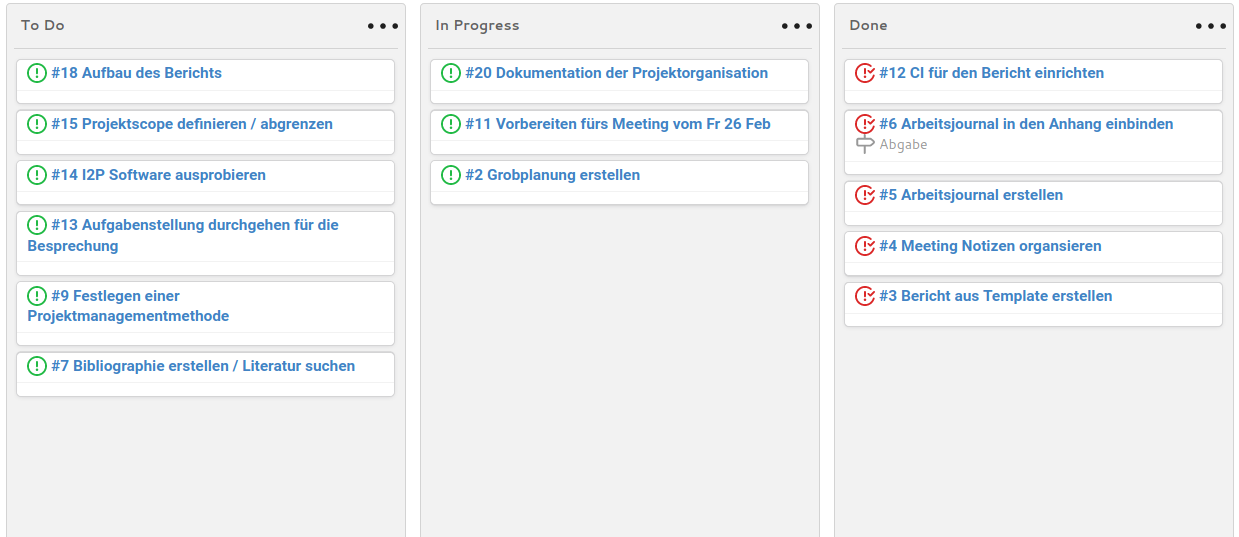
\includegraphics[width=1.0\textwidth]{project-board.png}
    \caption{CodeBerg Project Board}
    \label{fig:projectboard}
\end{figure*}

Ein einziger Issue sollte nie mehr Aufwand machen als acht Stunden Arbeit. Diese Regel hilft die Issues kleiner zu halten und genauere Aussagen treffen zu können, wo man im Projekt steht.
Wird an einem Issue gearbeitet wird dies im Arbeitsjournal vermerkt (siehe Anhang~\fulreff{sec:journal}).

\subsection{Projektanforderungen}
\label{sub:Anforderungen}

Die Anforderungen an das Projekt haben sich aus der Aufgabenstellung (siehe Anhang~\ref{ch:assignment}) sowie aus dem Requirements-Engineering durch regelmässige Meetings und Absprachen mit dem Auftraggeber ergeben. Die Vorgaben der Hochschule Luzern für Bachelorarbeiten wurden ebenfalls als Anforderungen aufgenommen.

Die folgende Tabelle~\ref{tab:anforderungen} zeigt alle ermittelten Anforderungen auf.
Die erste Spalte ''Id'' gibt jeder Anforderung einen eindeutigen Kennzeichner, um diese einfacher zu referenzieren.
Die Anforderung selber ist in der Spalte ``Anforderung'' genauer beschrieben.
Die Spalte ''Art'' gibt an, ob es sich bei der Anforderung um eine funktionale oder nicht-funktionale Anforderung handelt.
Nicht jede Anforderung muss zwingend erfüllt werden, deshalb kennzeichnet die Spalte ''Optional'', ob die jeweilige Anforderung zwingend erfüllt werden muss.

\begin{longtable}{N p{8.5cm} l l}
    \toprule
    \multicolumn{1}{r}{\bfseries Id} & \bfseries Anforderung                                                                                                                                                           & \bfseries Art & \bfseries Optional \\ \midrule
    \endhead
    \rid{SDTF}  & Der Stand der Technik/Forschung bezüglich I2P muss ermittelt und in den Bericht eingebunden werden.
                & Nicht-funktional & Nein  \\ \midrule


    \rid{TINF}  & Ein Teststand muss aufgebaut werden, welches es erlaubt verschiedene Performance-Messungen
                  an einem Netzwerk bestehend aus mehreren i2pd-Knoten auszuführen. & Funktional & Nein \\ \midrule
    \rid{TKON}  & Es soll ein Konzept erstellt werden für den Teststand. Dieser soll aufzeigen wie dieser aussehen soll, wie er funktioniert und was genau gemessen werden soll. & Nicht-funktional & Nein \\ \midrule
    \rid{TREP}  & Die am Teststand durchgeführten Messungen sollten so gut wie möglich reproduzierbar sein. Die gleiche Messung sollte soweit wie möglich dieselben Resultate liefern. & Nicht-funktional & Nein \\ \midrule
    \rid{TCNF}  & Gewisse Aspekte des Teststands und der i2pd-Knoten müssen konfigurierbar sein, damit verschiedene Messungen durchgeführt werden können.  & Funktional & Nein \\ \midrule
    \rid{TSCL}  & Der Teststand soll zwischen 8 bis maximal 256 i2pd-Knoten unterstützen. Dies muss konfigurierbar sein, um das I2P-Testnetzwerk für verschiedene Tests zu skalieren zu können. & Funktional & Nein \\ \midrule
    \rid{TISO}  & Das I2P-Testnetzwerk soll isoliert sein vom realen I2P-Netzwerk. & Nicht-funktional & Nein \\ \midrule
    \rid{TNET}  & Das I2P-Testnetzwerk soll als Knotenfamilie auch dem öffentlichen I2P-Netzwerk beitreten können. & Funktional & Ja \\ \midrule
    \rid{TLAT}  & Die Latenz von Nachrichten die über das I2P-Testnetzwerk gesendet werden, soll gemessen werden. & Funktional & Nein \\ \midrule
    \rid{TLIM}  & Es muss möglich sein im Teststand die verfügbare Bandbreite von einzelnen i2pd-Knoten einzustellen. & Funktional & Nein \\ \midrule
    \rid{TVRS}  & Man soll schnell (innerhalb von 2h) ein neues Experiment mit neuen Einstellungen starten können. & Nicht-funktional & Nein \\ \midrule
    \rid{EVAL}  & Die am Teststand durchgeführten Messungen müssen qualitativ evaluiert und aufgearbeitet werden.  & Nicht-funktional & Nein \\ \midrule
    \rid{TPER}  & Man geht davon aus, dass die Messungen lange dauern können, da jeweils ein ganzes Netzwerk und dessen Traffic erstellt und gehandhabt werden muss. Es ergibt Sinn, die Ausführungszeiten von Messungen kurz zu halten, damit mehr Messungen durchgeführt werden können. & Nicht-funktional & Ja \\ \midrule
    \rid{DOCS}  & Am Ende des Projekts muss diese Bachelorarbeit abgegeben werden. Der Bericht soll das Projekt, die verwendeten Methoden, Evaluationsprozesse, Umsetzung und Resultate beschreiben.
                & Nicht-funktional & Nein \\ \midrule
    \rid{ITER}  & Ein iteratives Projektmanagement wird bevorzugt für kurze Feedback-Zyklen. & Nicht-funktional & Ja \\ \midrule
    \rid{PRES}  & Es muss eine Zwischenpräsentation vorgetragen werden, welche das Projekt und das weitere Vorgehen erklärt.
                & Nicht-funktional & Nein \\ \midrule
    \rid{WEBA}  & Es muss ein Web-Abstract erstellt werden, der das Projekt kurz zusammenfasst. Der Web-Abstract wird veröffentlicht und muss eine Woche vor Projektende vom Betreuer abgenommen werden.
                & Nicht-funktional & Nein \\ \midrule
    \rid{PVID}  & Es muss ein 90 Sekunden Video erstellt werden, welches diese Bachelorarbeit kurz erklärt. Das Video wird am Start der Schlusspräsentation abgespielt.
                & Nicht-funktional & Nein \\ \midrule
    \bottomrule
    \caption{Anforderungen}\label{tab:anforderungen}
\end{longtable}

\subsection{Planung}
\label{sec:Planung}

Für diese Bachelorarbeit werden 360 Stunden Arbeit während den 15. Projektwochen geleistet.
Im Schnitt bedeutet dies acht Stunden Arbeit an jeweils drei Wochentagen (meistens jeweils Mittwoch-Freitag).
Neben den definierten Meilensteinen, Projektphasen und dem Projektkalender gibt es auch eine Liste an Resultaten im Anhang~\ref{ch:resultate}, welche eine Zeitschätzung für jedes Projektresultat beinhaltet.

% 15 Wochen * 3 Tage * 8h = 360h

\subsubsection{Meilensteine}
\label{sec:meilensteine}

Die Meilensteine sind im Projektkalender (\fullref{tab:projektkalender}) hellblau gekennzeichnet und hier aufgelistet.

\begin{enumerate}[itemsep=0]
    \item \textbf{Startdatum}: Mittwoch, 24. Februar 2021, Kick-Off-Meeting
    \item \textbf{Zwischenpräsentation}: 21. April 2021, 14:00
    \item \textbf{Abgabe Web-Abstract}: 28. Mai 2021
    \item \textbf{Abgabedatum}: Ursprünglich 4. Juni 2021, verschoben auf 20. September, 12:00
    \item \textbf{Schlusspräsentation}: Ursprünglich 26. Juni 2021, 14:00, verschoben auf 29. September, 16:00
\end{enumerate}

Die Meilensteine sollen ein Controlling-Mechanismus sein, um feststellen zu können, wenn das Projekt im Verzug ist.
Diese Meilensteine wurden auch in den Issue-Tracker aufgenommen:\\
\url{https://codeberg.org/mkuettel/BA/milestones}

\subsubsection{Phasen}
\label{sec:phasen}

Das Projekt wird in vier Phasen durchgeführt, welche in Tabelle \fullref{tab:projektkalender} dargestellt sind.
Dabei sind die Phasen jeweils durch Meilensteine voneinander abgegrenzt.

\begin{enumerate}[itemsep=0]
    \item \textbf{Konzeptionsphase}: Die Konzeptionsphase beginnt mit dem Kick-Off Meeting.
        In dieser Phase wird das Projekt geplant, recherchiert, der Bericht wird strukturiert, die Anforderungen werden eruiert und  ein Konzept für einen Teststand wird erstellt.
    \item \textbf{Aufbau des Teststands}: Ein Teststand aufbauen nach Konzept um Performance-Experimente und Messungen mit der i2pd-Software in einem Netzwerk machen zu können.
    \item \textbf{Auswertungsphase}: Verschiedene Performance-Experimente und Messungen werden in dieser Phase ausgeführt und ausgewertet.
    \item \textbf{Abschlussphase}: Vervollständigen des Berichts, Fazit erstellen, Korrekturlesen, Erstellung des Web-Abstracts.
\end{enumerate}

\subsubsection{Projektkalender}

Die folgende Tabelle~\fullref{tab:projektkalender} war enorm hilfreich um die Übersicht während des Projekts zu behalten.
Die Spalte ''PW'' gibt die Projektwoche an, die Spalte ''KW'' die Kalenderwoche.

\newcommand{\cellblue}[1]{\cellcolor{cyan} #1}
\begin{table}[H]
    \begin{tabular}{r r l l|c c|c c c|c c}
        \toprule
         \textbf{PW} & \textbf{KW}      & \textbf{Phase} & \textbf{Meilensteine} & \multicolumn{7}{c}{\textbf{Wochentag}} \\
                     &            &                       &                       & \textbf{Mo} & \textbf{Di} & \textbf{Mi}  & \textbf{Do} & \textbf{Fr} & \textbf{Sa} & \textbf{So} \\ \midrule
                           &                         &                       &                       & \multicolumn{7}{c}{\textit{Februar}}   \\
          1                & 8                       & \textbf{Konzeption}         & Projektstart          & 22                                      & 23 & \cellblue{24}  & 25 & 26 & 27 & 28 \\
                           &                         &                       &                       & \multicolumn{7}{c}{\textit{März}}      \\
          2                & 9                       &                       &                       & 1                                       & 2  & 3   & 4  & 5  & 6  & 7  \\
          3                & 10                      &                       &                       & 8                                       & 9  & 10  & 11 & 12 & 13 & 14 \\
          4                & 11                      &                       & 1. Konzept Teststand     & 15                                      & 16 & 17  & 18 & 19 & 20 & 21 \\
          \midrule
          5                & 12                      & \textbf{Aufbau des}          &                       & 22                                      & 23 & 24  & 25 & 26 & 27 & 28 \\
          6                & 13                      & \textbf{Teststands}            &                       & 29                                      & 30 & 31  &    &    &    &    \\
          |                & |                       &                       &                       & \multicolumn{7}{c}{\textit{April}}     \\
          6                & 13                      &                       &                       &                                         &    &     & 1  & 2  & 3  & 4  \\
          7                & 14                      &                       &                       & 5                                       & 6  & 7   & 8  & 9  & 10 & 11 \\
          8                & 15                      &                       & 2. Zwischenpräsentation  & 12                                      & 13 & 14  & 15 & 16 & 17 & 18 \\
          \midrule
          9                & 16                      & \textbf{Auswertung}         &                       & 19                                      & 20 & \cellblue{21}  & 22 & 23 & 24 & 25 \\
          10               & 17                      &                       &                       & 26                                      & 27 & 28  & 29 & 30 &    &    \\
          |                & |                       &                       &                       & \multicolumn{7}{c}{\textit{Mai}}       \\
          10               & 17                      &                       &                       &                                         &    &     &    &    & 1  & 2  \\
          11               & 18                      &                       & 3. Auswertung            & 3                                       & 4  & 5   & 6  & 7  & 8  & 9  \\
          \midrule
          12               & 19                      & \textbf{Abschluss}             &                       & 10                                      & 11 & 12  & 13 & 14 & 15 & 16 \\
          13               & 20                      &                       & 4. Web-Abstract          & 17                                      & 18 & 19  & 20 & 21 & 22 & 23 \\
          14               & 21                      &                       &                          & 24                                      & 25 & 26  & 27 & \cellblue{28} & 29 & 30 \\
          15               & 22                      &                       &                       & 31                                      &    &     &    &    &    &    \\
           |               & |                       &                       &                       & \multicolumn{7}{c}{\textit{Juni}}      \\
          15               & 22                      &                       & 5. Abgabe                &                                         & 1  & 2   & 3  & \cellblue{4} & 5  & 6  \\
        \bottomrule
    \end{tabular}

    \caption{Projektkalender}
    \label{tab:projektkalender}
\end{table}

Es gilt zu beachten das dies eine Planung ist. Der effektive Projektverlauf ist im Issue-Tracker und im Arbeitsjournal im Anhang~\ref{sec:journal} ersichtlich.
Aus gesundheitlichen Gründen wurden die letzten beiden Projektwochen in den September verschoben.


